%This has additional interest in that, not only does it probe the \fcnc, but the \kpipi system can
%result from the decay of numerous strange resonances.

The decays \btokpipimumu and \btophikmumu both are \decay{\bquark}{\squark\mumu} \fcnc
transitions, which are forbidden at tree level in the \sm\footnote{All mentions of the \phii
  refer implicitly to the $\phi(1020)$ meson.
}.
Therefore, these processes are sensitive to virtual \np particles contributing
to the decay amplitude in loops.
%Figure~\ref{fig:hhh:feyn} shows the pengiun diagrams which propagate these decays in the SM.


%%%%%%%%%%%%%%%%%%%%%%%%%%%%%%%%%%%%%%%%%%%%%%%%%%%%%%%%%%%%%%%%%%%%%%%%%%%%%%%%%%%%%%%%%%%%%%%%%%
%\subsection[Operator product expansion for \btokpipimumu and \btophikmumu]
%{Operator product expansion for $\boldsymbol{\btokpipimumu}$ and $\boldsymbol{\btophikmumu}$}
%%%%%%%%%%%%%%%%%%%%%%%%%%%%%%%%%%%%%%%%%%%%%%%%%%%%%%%%%%%%%%%%%%%%%%%%%%%%%%%%%%%%%%%%%%%%%%%%%%

\begin{figure}
  \begin{center}
    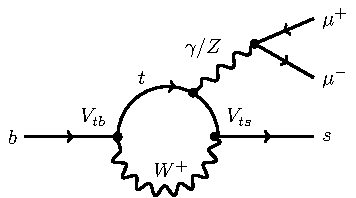
\includegraphics[scale=1]{feynman_btosmumu_penguin}
    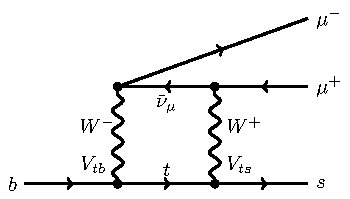
\includegraphics[scale=1]{feynman_btosmumu_box}
    \caption[Schematic Feynman diagrams for loop and box diagrams]
    {
      Schematic Feynman diagrams for the operators \Op7, \Op9, and \Op{10} which are most sensitive
      to the \decay{\bquark}{\squark\mumu} \fcnc.
      The propagators are the (left) photonic and $Z$ penguin diagram, and the (right) \Wp mediated
      box diagram.
      Operator \Op7 describes the photonic pengiuin diagram; while \Op9 and \Op{10} are the
      vector and axial-vector parts of both the $Z$ and \Wp diagrams.
      %Operators (left) \Op7 and \Op9 are the photon and $Z$ mediated penguin diagrams, respectively.
      %The operator \Op{10} (right) is the box diagram for the same transition.
    }
    \label{fig:hhh:loops}
  \end{center}
\end{figure}

Transitions of the \fcnc $\decay{b}{s\ell^+\ell^-}$ can be expressed with the effective Hamiltonian
\begin{equation}
  \Ham{eff} = -4\frac{G_F}{\sqrt{2}}\Vconj{ts}\V{tb}\frac{e^2}{16\pi^2}
  \sum_{i=1}^{10}\big[C_i(\Lambda)\mathcal{O}_i(\Lambda)
    +C_i^\prime(\Lambda)\mathcal{O}_i^\prime(\Lambda)\big],
\end{equation}
as in \Eq{eq:th:opeham}. %, where the coefficients are known as Wilson coefficients, which
%correspond to the Wilson operators $\mathcal{O}_{1-10}$.
Operators which are particularly sensitive to NP contributions in \decay{b}{s\mumu} transitions are
\begin{align}
  \Op{7\pz} &= \frac{m_b}{e}\big(\bar\squark\sigma_{\mu\nu}P_Rb\big)F^{\mu\nu}
  %$\bra{f}\Op}\ket{i}$.
  &\Op{7\pz}^\prime &= \frac{m_b}{e}\big(\bar s \sigma_{\mu\nu}P_Lb\big)F^{\mu\nu}
  \nonumber\\
  %\mathcal{O}_8 &= g\frac{m_b}{e^2}\big(\bar s \sigma_{\mu\nu}T^aP_Rb\big)G^{\mu\nu a}
  %&\mathcal{O}_8^\prime &= g\frac{m_b}{e^2}\big(\bar s \sigma_{\mu\nu}T^aP_Rb\big)G^{\mu\nu a}
  %\\
  \Op{9\pz} &= \big(\bar s\gamma_\mu P_Lb\big)\big(\bar\ell\gamma^\mu\ell\big)
  &\Op{9\pz}^\prime &= \big(\bar s\gamma_\mu P_Rb\big)\big(\bar\ell\gamma^\mu\ell\big)
  \nonumber\\
  \Op{10} &= \big(\bar s\gamma_\mu P_Lb\big)\big(\bar\ell\gamma^\mu\gamma_5\ell\big)
  &\Op{10}^\prime &= \big(\bar s\gamma_\mu P_Rb\big)\big(\bar\ell\gamma^\mu\gamma_5\ell\big).
  %\phantom{\frac{1}{1}}
  %\mathcal{O}_{S} &= \frac{m_b}{m_{B_s}}\big(\bar s\gamma_\mu P_Rb\big)\big(\bar\ell\ell\big)
  %\mathcal{O}_{P} &= \frac{m_b}{m_{B_s}}\big(\bar s\gamma_\mu P_Rb\big)\big(\bar\ell\gamma_5\ell\big)
\end{align}
The operator \Op7 describes the transition of \decay{\bquark}{\squark\gamma}, in the \sm this is
via a photonic penguin diagram.
Operators \Op9 and \Op{10} are the vector and axial-vector components of the four point
\decay{\bquark}{\squark\mumu} interaction; in the \sm these operators are made up of the $Z$
mediated penguin, and the \Wp box diagrams.
%The operators \Op7 and \Op9 describe the \fcnc via vector and axial vector transitions.
%In the \sm the vector operator is due to the photonic penguin diagram, and the axial vector is the
%same schematic diagram with a mediating $Z$.
%Operator \Op{10} corresponds to the \emph{box} diagram for with mediating \Wp bosons.
A penguin diagram is so called, because if one draws it on top of a picture of a penguin, it looks
like a penguin.
Figure~\ref{fig:hhh:loops} shows schematic Feynman diagrams for \Op7, \Op8, and \Op{10}.
Primed operators are the suppressed helicity (usually right-handed), whose contributions are
vanishingly small in the \sm.
The operators \Op{1-6} encapsulalong distance contributions, such as \ccbar
loops, and \Op{8} is the gluonic penguin operator.

%%%%%%%%%%%%%%%%%%%%%%%%%%%%%%%%%%%%%%%%%%%%%%%%%%%%%%%%%%%%%%%%%%%%%%%%%%%%%%%%%%%%%%%%%%%%%%%%%%
%%%%%%%%%%%%%%%%%%%%%%%%%%%%%%%%%%%%%%%%%%%%%%%%%%%%%%%%%%%%%%%%%%%%%%%%%%%%%%%%%%%%%%%%%%%%%%%%%%

Both decays \btokpipimumu and \btophikmumu proceed via a \decay{\bquark}{\squark\mumu} \fcnc with a
spectator \uquark quark, the decays mediated by penguin loops are shown in \Fig{fig:hhh:feyn}.
In this way, both these decays are the same as the \fcnc decay $\decay{\Bd}{K^{*0}\mumu}$, but
differ in the \qqbar pairs that are popped from the QCD field.
There is considerable interest surrounding the decay $\decay{\Bd}{K^*(892)^0\mumu}$, becuase
not only is it an \fcnc, but its angular distributions provide complementary sensitivity to \np.
Furtheremore, a $3.7\stdev$ deviation is observed in the $P_5^\prime$ parameter in \lhcb data in
comparison to theoretical predictions~\cite{LHCb-CONF-2015-002}.



%has similarities with the decay $\decay{\Bp}{K^*(892)^0\mumu}$.
%Both propagate in the same way, but the latter's final state is $\kpi\mumu$ --- the decay
%\btokpipimumu requires an additional \uubar pair.

\begin{figure}
  \begin{center}
    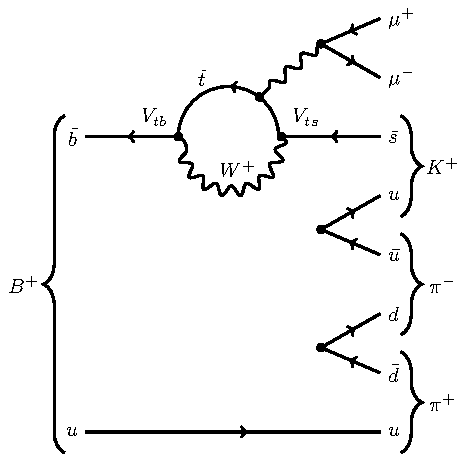
\includegraphics[scale=1]{feynman_hhh_kpipimumu}
    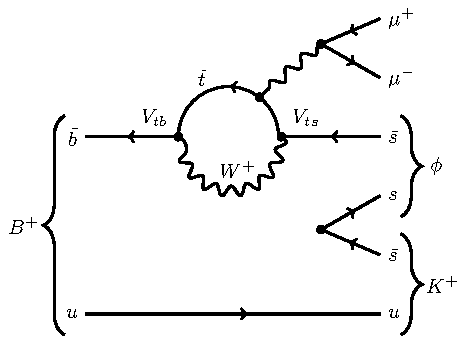
\includegraphics[scale=1]{feynman_hhh_phikmumu}
    \caption[Feynman diagrams for \btokpipimumu and \btophikmumu]
    {
      Feynman diagrams illustrating how the decays \btokpipimumu and \btophikmumu can proceed in
      the SM via operators \Op7, \Op9 and \Op{10}.
      The operators \Op{1-6} also contribute a small amount.
    }
    \label{fig:hhh:feyn}
  \end{center}
\end{figure}

In the decay \btokpipimumu, the structure of the \kpipi system's mass distribution results from the
decay of a variety of strange resonances.
Contributions of resonances to the \kpipi system has been previously studied by the \belle
collaboration in the tree level decay \btojpsikpipi, where \jpsitomumu~\cite{Guler:2010if}.
This study indicated that the dominant contribution to the \kpipi system should be expected
to be from decaying \kone{1270} mesons.
The total brancing fraction of the decay \decay{\kone{1270}}{\kpipi}
%The \kone{1270} decays into the \kpipi final state
--- via both a non-resonant decay and various resonances ---
with a branching fraction of
$\BF\big(\decay{\kone{1270}}{\kpipi}\big)=\big(35.7\pm3.7\big)\,\%$~\cite{PDG2012}.
The \kone{1270} meson, together with the \kone{1400}, are mass eigenstates resulting from the
mixing of the $P$-wave axial vector states $K_{1A}(1^3P_1)$ and $K_{1B}(1^1P_1)$ according to:
\begin{equation}
  \begin{pmatrix}
    \ket{\kone{1270}} \\
    \ket{\kone{1400}}
  \end{pmatrix}
  =
  \begin{pmatrix}
    \sinthetakone & \costhetakone \\
    \costhetakone & -\sinthetakone
  \end{pmatrix}
  \begin{pmatrix}
    \ket{K_{1A}^+} \\
    \ket{K_{1B}^+}
  \end{pmatrix}.
  \label{eq:k1mixing}
\end{equation}
Here, \thetakone is the mixing angle and has been measured to have central values of both $-34^\circ$ and
$-57^\circ$~\cite{PhysRevD.47.1252,Tayduganov:2011ui,Hatanaka:2008xj,Cheng:2011pb,Divotgey:2013jba,Cheng:2013cwa}.
However, more recent measurements favour a value of
$-(34\pm13)^\circ$~\cite{Hatanaka:2008xj,Cheng:2011pb,Divotgey:2013jba,Cheng:2013cwa},
and the most recent rule out the solution at $-57^\circ$ entirely~\cite{Divotgey:2013jba,Cheng:2013cwa}
(but with a different sign convention).

Due to the unknown composition of the \mass{\kpipi} spectrum, an inclusive prediction of the
branching fraction $\BF(\btokpipimumu)$ does not exist.
However, the branching fraction of the rare decay \decay{\Bp}{\kone{1270}\mumu} is predicted to
be~\cite{Hatanaka:2008gu}
\begin{equation}
  \BF\big(\decay{\Bp}{\kone{1270}\mumu}\big) = \big(2.3\,^{+1.3}_{-1.0}\,^{+0.0}_{-0.2}\big)\e{-6},
\end{equation}
where uncertainties arise from form-factor calculations and the mixing angle, respectively.

Figure~\ref{fig:th:thetak1} shows the theoretical \qsq distribution for the decay
$\decay{\Bp}{K_1^+\mumu}$, for both the \kone{1270} and \kone{1400} and varying \thetakone.
The \decay{b}{s\mumu} can be mediated by a virtual photon which, for some values of \thetakone, can
be transversely polarized.
However, for some values of \thetakone the \mumu pair is fully longitudinally polarized and the
decay via a photon is forbidden.

\begin{figure}
  \begin{center}
    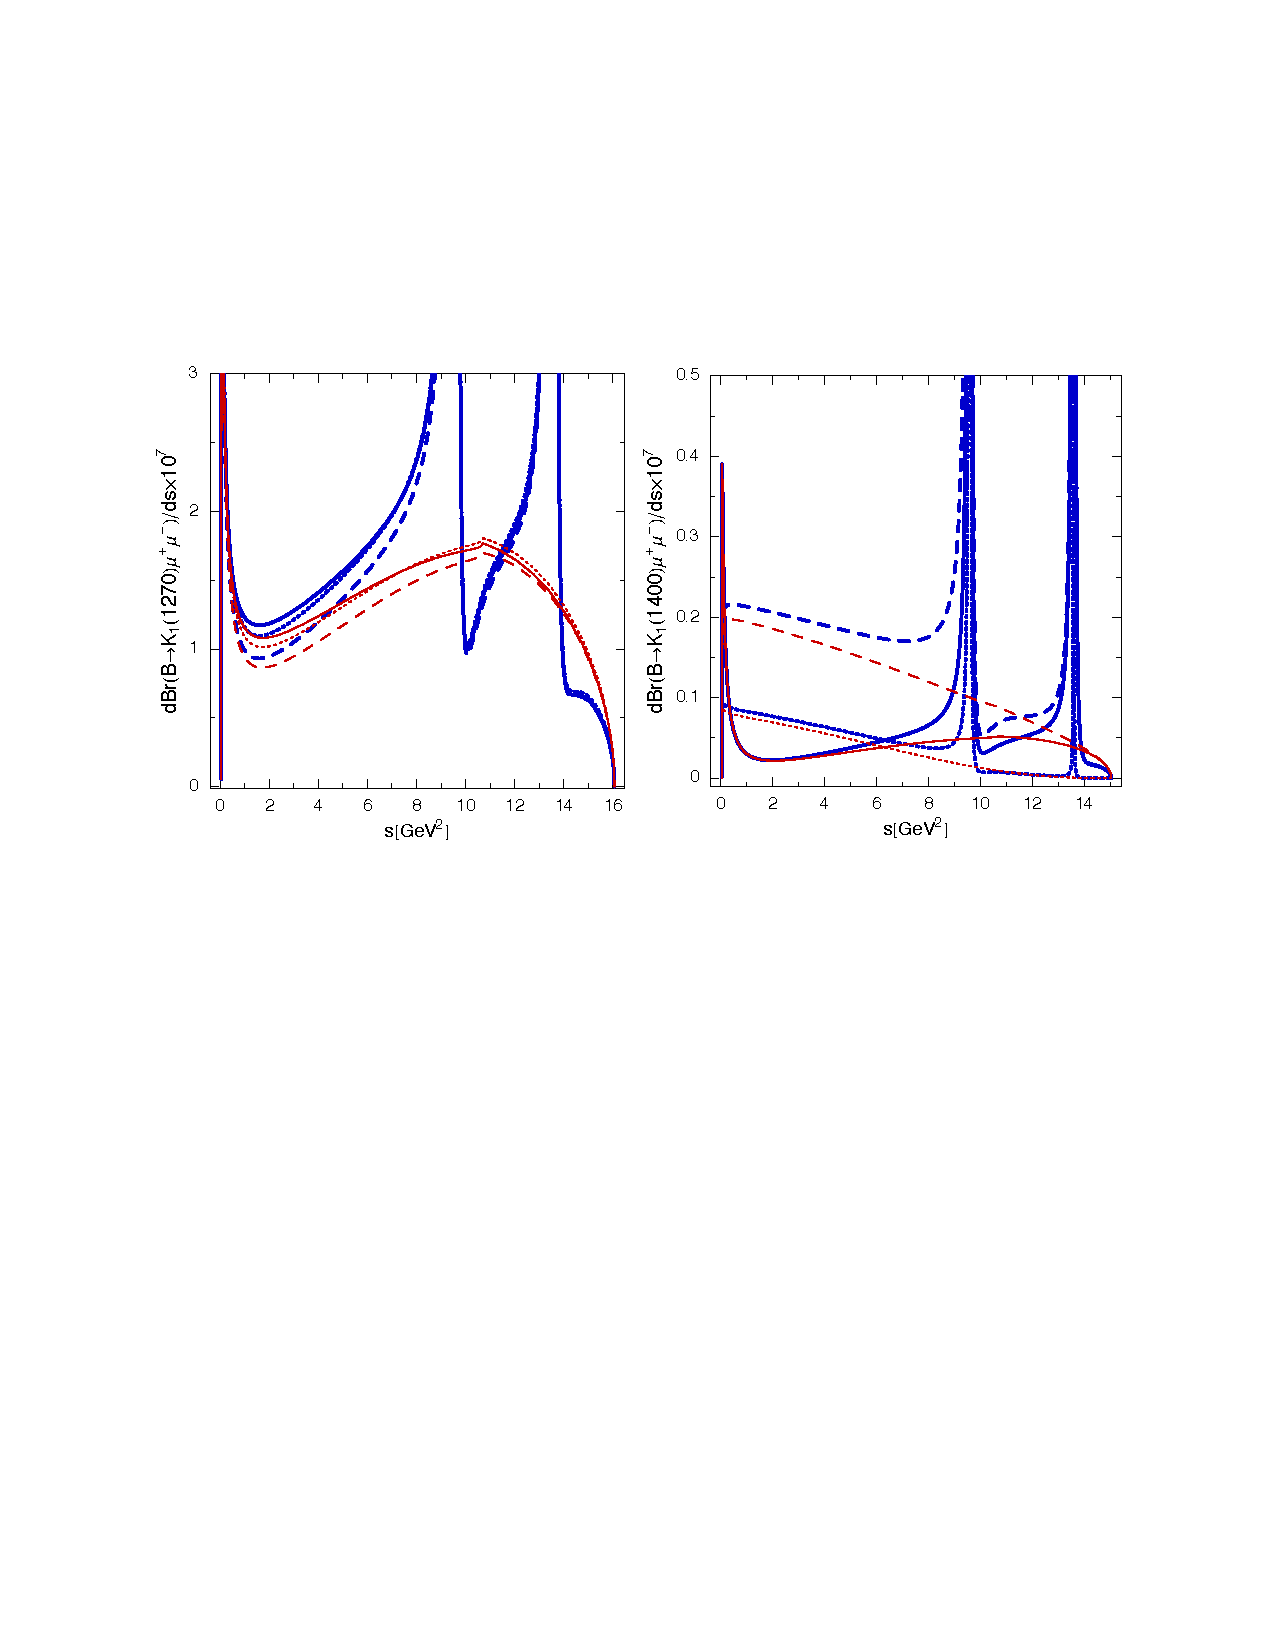
\includegraphics[width=0.96\textwidth]{K1_q2_theory}
    \caption[Theoretical \qsq distribution for $\decay{\Bp}{K_1^+\mumu}$]
    {
      The dimuon invariant mass distributions for the differential decay rates, as taken from
      \Ref{Hatanaka:2008gu}.
      $\dBF(\decay{\Bp}{K_1^+\mumu})/\dqsq$, (where $s=\qsq$), for the \kone{1270} and \kone{1400}.
      Central values of input form factors are used.
      The thick blue lines and thin red curves indicate the differential branching fractions with
      an without corrections from resonances, respectively.
      Solid, dotted and dashed lines correspond to values of the mixing angle
      $\thetakone=-34^\circ,-45^\circ,-57^\circ$ respectively.
    }
    \label{fig:th:thetak1}
  \end{center}
\end{figure}

There are no predictions for the branching fraction of the decay \btophikmumu,
but one would expect it to be smaller than that of the decay \btokpipimumu.
This is becuase it requires an \ssbar to be created from the QCD field rather than a \uubar and
\ddbar pair.

Absent from this analysis are the searches for the decays \decay{\Bp}{\Kp\Km\pip\mumu}
and \decay{\Bp}{\pipi\pim\mumu}.
These were not included because they are suppressed by a factor of $|\V{td}/\V{ts}|^2\simeq23$ and
suffer from large backgrounds.

The following chapter outlines an analysis of the decays \btokpipimumu and \btophikmumu in which
branching fractions for each decay is measured.
Also, a measurement of the differential branching fraction of \btokpipimumu is made in bins of
\qsq; where \qsq is the invariant mass of the dimuon object squared.






%HADRONIC UNCERTAITIES
%HADROMIZAITON
